\documentclass{article}
\usepackage[utf8]{inputenc}
\usepackage[portuges]{babel}
\usepackage[a4paper, total={7in, 9in}]{geometry}
\usepackage{graphicx}
\usepackage{float}
\usepackage[style=numeric]{biblatex}
\usepackage{csquotes}
\usepackage{fancyvrb}
\usepackage{subcaption}
\usepackage{listings,color}

\definecolor{light-gray}{gray}{0.95}

\lstset{
    basicstyle=\fontsize{9}{11}\ttfamily,
    backgroundcolor=\color{light-gray},
    breaklines=true,
    extendedchars=true,
    inputencoding=utf8,
    literate=
    {á}{{\'a}}1 {é}{{\'e}}1 {í}{{\'i}}1 {ó}{{\'o}}1 {ú}{{\'u}}1
    {Á}{{\'A}}1 {É}{{\'E}}1 {Í}{{\'I}}1 {Ó}{{\'O}}1 {Ú}{{\'U}}1
    {ã}{{\~a}}1 {ẽ}{{\~e}}1 {ĩ}{{\~i}}1 {õ}{{\~o}}1 {ũ}{{\~u}}1
    {Ã}{{\~A}}1 {Ẽ}{{\~E}}1 {Ĩ}{{\~I}}1 {Õ}{{\~O}}1 {Ũ}{{\~U}}1
    {à}{{\`a}}1 {è}{{\`e}}1 {ì}{{\`i}}1 {ò}{{\`o}}1 {ù}{{\`u}}1
    {À}{{\`A}}1 {È}{{\'E}}1 {Ì}{{\`I}}1 {Ò}{{\`O}}1 {Ù}{{\`U}}1
    {â}{{\^a}}1 {ê}{{\^e}}1 {î}{{\^i}}1 {ô}{{\^o}}1 {û}{{\^u}}1
    {Â}{{\^A}}1 {Ê}{{\^E}}1 {Î}{{\^I}}1 {Ô}{{\^O}}1 {Û}{{\^U}}1
    {ç}{{\c c}}1 {Ç}{{\c C}}1
}

\addbibresource{references.bib}


\newcommand{\titleRule}{
    \rule{\linewidth}{0.5mm} \\ [0.25cm]
}

\begin{document}

\begin{titlepage}
    \center
    \begin{figure}[H]
        \centering
        
\includegraphics[width=4cm]{Pictures/UM_EENG.jpg}
    \end{figure}
    \textsc{\LARGE Universidade do Minho} \\ [1.5cm]
    \textsc{\Large Mestrado Integrado em Engenharia Informática} \\ [0.5cm]
    \textsc{\large Processamento de Dados com Streams de Java} \\ [0.5cm]

    \titleRule
    {\huge \bfseries Análise de \textit{performance} de Streams de Java}
    \titleRule

    João Pedro Ferreira Vieira A78468 \\
    Miguel Miranda Quaresma A77049 \\
    Simão Paulo Leal Barbosa A77689 \\[0.25cm]

    \today
\end{titlepage}

\tableofcontents

\newpage

\section{Introdução}
A realização de \textit{benchmarks} é uma prática comum quando se pretende otimizar uma aplicação. Estas otimizações podem ser realizadas em diversas componentes 
do sistema sendo útil determinar qual a forma mais eficiente de realizar uma dada operação. Para tal é indispensável dispor de ferramentas e metodologias que 
permitam avaliar o tempo de execução de frações de código reduzidas, sendo este um processo designado por \textit{Microbenchmarking}(\cite{microbenchmarking}).
O presente trabalha apresenta o resultado de um conjunto de \texttt{microbenchmarks} relativas à utilização de \texttt{Streams} e outros iteradores de coleções
em Java (\texttt{Iterator<T>, forEach, for}) no processamento de grandes quantidades de dados e pretende determinar quais destas implementações apresentam melhor 
\textit{performance} no tratamento de quantidades massivas de dados. São ainda realizadas comparações entre processamento paralelo vs. sequencial no uso de 
\texttt{Streams} bem como entre as versões Java 8 e 9.



\section{Framework de testes - Especificações de Hardware}
Os resultados de \textit{benchmarks} são influenciados pelo contexto em que são realizadas, nomeadamente a plataforma de \textit{hardware} utilizada e os métodos estatísticos 
usados na recolha e tratamento de dados, tornando-se útil apresentar uma breve descrição deste contexto.

\subsection{Plataforma de Hardware}
A máquina usada para realizar as benchmarks especificadas apresenta as seguintes configurações:
\begin{itemize}
    \item \textbf{Marca}: Asus
    \item \textbf{Modelo}: S510UN-78A94DB1
    \item \textbf{CPU}: Intel Core i7-8550U
        \begin{itemize}
            \item \textbf{\#Cores}: 4
            \item \textbf{Frequência}: 1.80 GHz
            \item \textbf{Cache}: 8MB
        \end{itemize}
    \item \textbf{Memória RAM}: 8GB
\end{itemize}

\subsection{Metodologia de testes}
Por forma a obter valores normalizados, precisos, reproduzíveis e limitar a influência de \textit{outliers} nos valores considerados foram
recolhidas, para cada benchmark, 15 amostras e o valor da mediana tomado como o tempo de execução para a configuração correspondente.
Adicionalmente, por forma a automatizar a realização de testes, foi desenvolvido o método \texttt{testeBoxGen}, com a seguinte assinatura:

\begin{lstlisting}
public static <R> SimpleEntry<Double,R> testeBoxGen(Supplier<? extends R> supplier)
\end{lstlisting}

que, dado um fornecedor de resultados, realiza um teste e devolve o tempo de execução e o resultado da mesma. Foi também desenvolvido o método \texttt{sampler}:

\begin{lstlisting}
private static <R> Double sampler(Supplier<? extends R> supplier)
\end{lstlisting}

que se encarrega de recolher 15 amostras do tempo de execução para cada \texttt{Supplier} e devolve a mediana desses tempos:

\begin{lstlisting}
List<Double> samples = new ArrayList<>(); 
    
for(int i = 0; i < 15; i ++){
    Crono.start();
    resultado = supplier.get();
    tempo = Crono.stop();
    samples.add(tempo);
}

Collections.sort(samples);

pivot = samples.size() / 2;

if(samples.size() % 2 == 0)
    return samples.get(pivot);
else return (samples.get(pivot) + samples.get(pivot+1))/2;
\end{lstlisting}

Os testes foram realizados processando ficheiros que continham informação referente a transações (financeiras), variando no número de transações que cada um continha: $1e6$, $2e6$, $4e6$, $6e6$.

\section{Análise de resultados}
\subsection{Benchmark T1}
A primeira \textit{benchmark} realizada consiste em processar os valores correspondentes a cada uma das transações e calcular a sua soma e média.
As implementações analisadas variam na estrutura de dados e forma de percorrer a mesma, nomeadamente: 
\begin{itemize}
    \item \textit{array} de \texttt{Doubles} \texttt{Double[]} percorrido através de um \textit{loop} \texttt{for} e de um iterador externo \texttt{forEach}
    \item \texttt{DoubleStream} Sequencial e Paralela
    \item \texttt{Stream<Double>} Sequencial e Paralela
\end{itemize}
\begin{figure}[H]
    \centering
    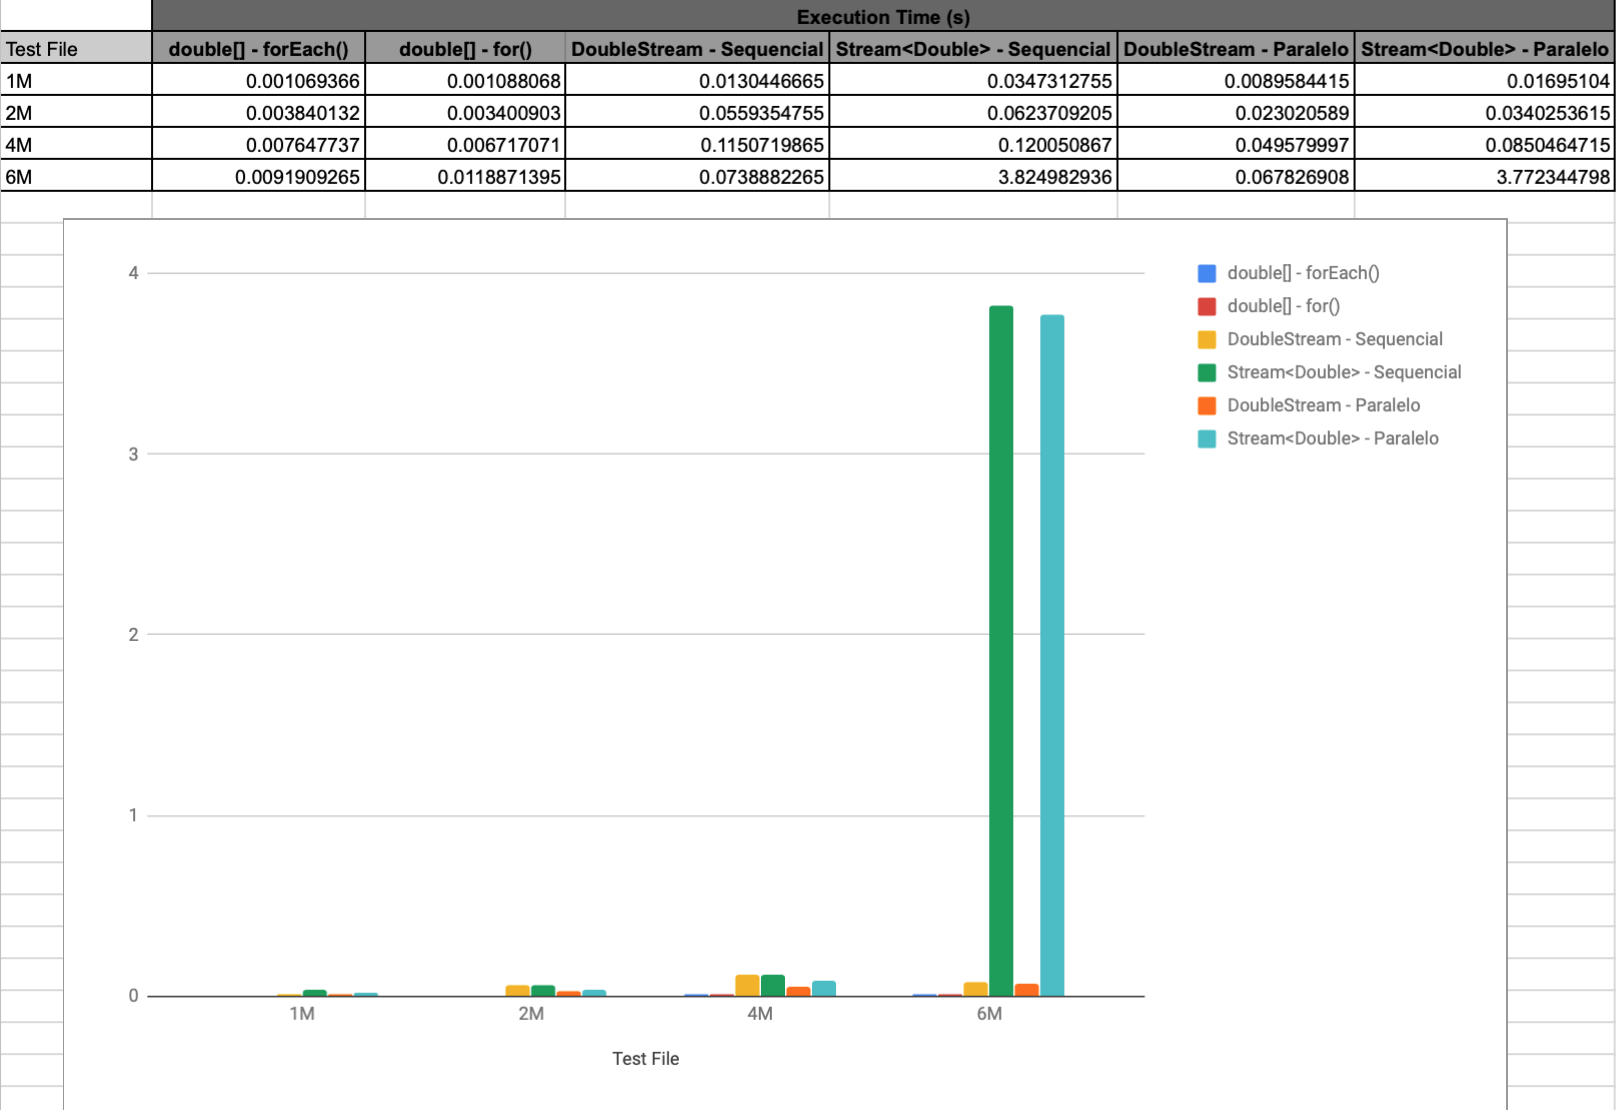
\includegraphics[width=10cm]{Pictures/T1.png}
    \caption{Benchmark T1 - Soma}
\end{figure}
Uma observação atenta dos dados recolhidos permite identificar diversos aspetos importantes. Um destes aspetos que deve ser mencionado trata-se da diferença de 
\textit{performance} entre \texttt{Streams} especializadas, neste caso \texttt{DoubleStream}, e genéricas, \texttt{Stream<Double>} causada pelo facto
de que, quando são usados tipos primitivos de dados como \texttt{Integer}, \texttt{Double} e \texttt{Long}, as \texttt{Streams} genéricas exigem o \texttt{boxing}
dos seus elementos que resulta na deterioração da \textit{performance} resultante.

\begin{figure}[H]
    \centering
    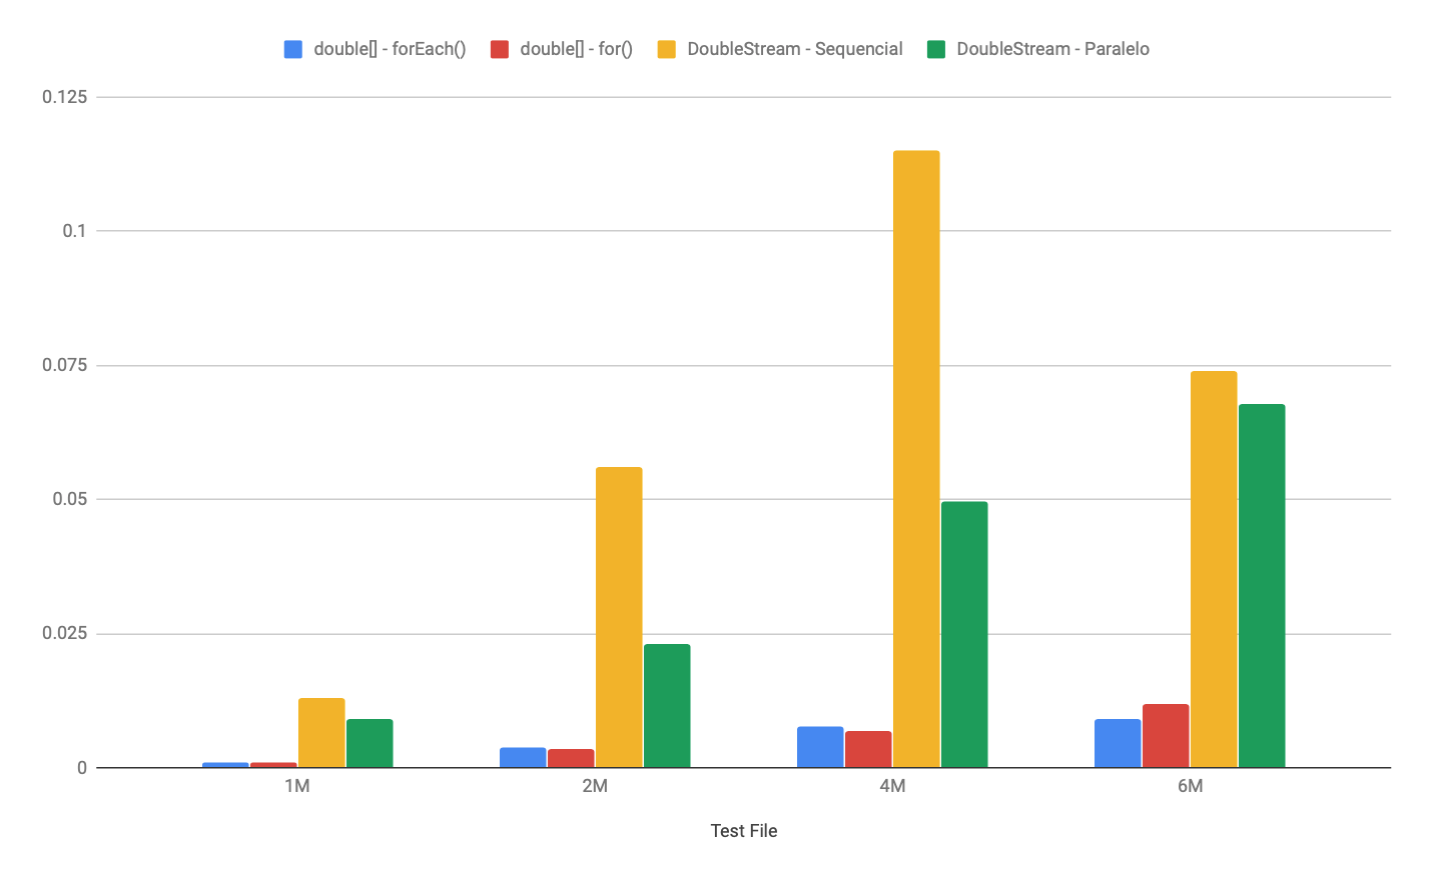
\includegraphics[width=10cm]{Pictures/T1_1.png}
    \caption{Benchmark T1 - Soma: double[] vs. DoubleStream}
\end{figure}

A comparação entre \texttt{DoubleStreams} e \texttt{double[]} permite observar um padrão interessante, mesmo com o aumento no volume de dados, o segundo apresenta uma 
\textit{performance} superior. Uma das razões reside na localidade de dados dos \textit{arrays} que correspondem a regiões contíguas de memória e permitem explorar a 
localidade espacial nos dados, algo apenas tornado possível por se tratarem de dados primitivos(\texttt{double}) e não de objetos, como é o caso das 
\texttt{DoubleStreams} (\texttt{Double}).

As mesmas conclusões podem ser retiradas do cálculo da média, como se pode observar pelos resultados ilustrados:


\begin{figure}[H]
\centering
\begin{subfigure}{.5\textwidth}
  \centering
  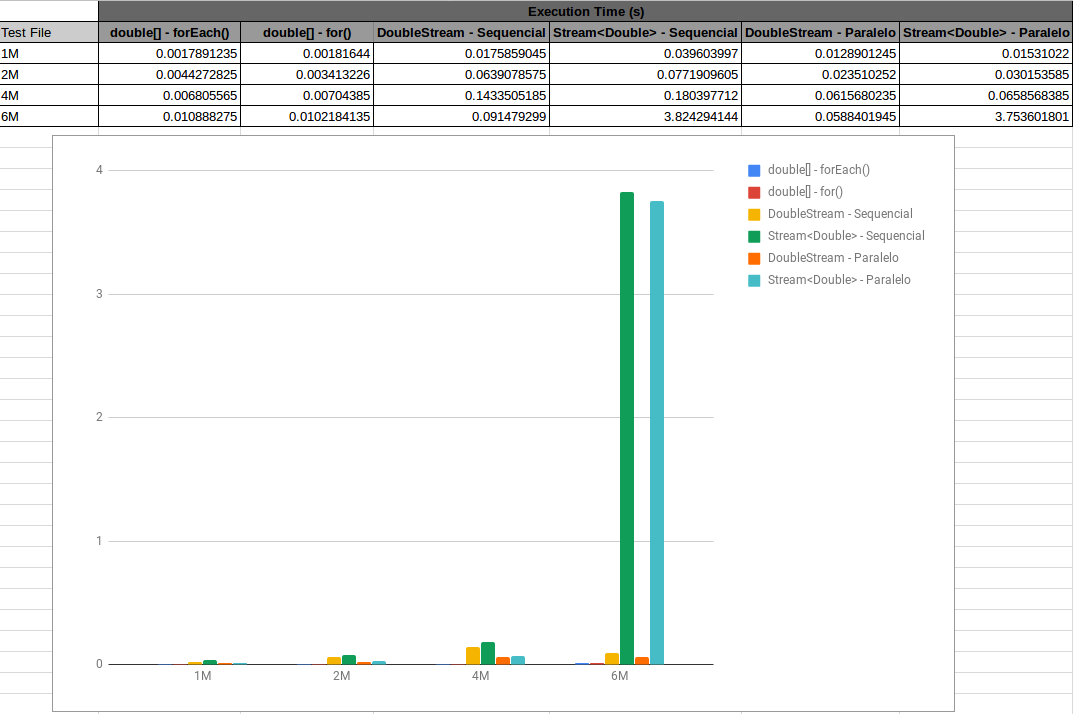
\includegraphics[width=1\linewidth]{Pictures/T1_2.png}
\end{subfigure}%
\begin{subfigure}{.5\textwidth}
  \centering
  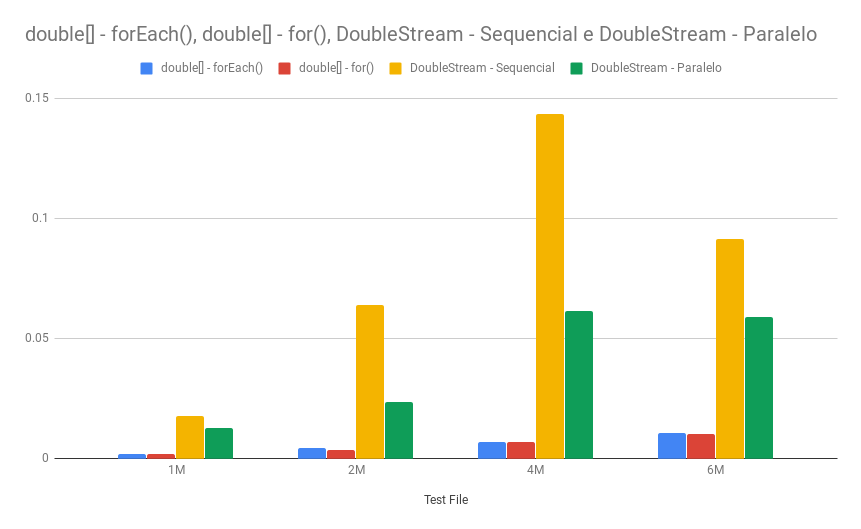
\includegraphics[width=1\linewidth]{Pictures/T1_3.png}
\end{subfigure}
\caption{Resultados do Benchmark T1 para cálculo da média}
\label{fig:sharedt}
\end{figure}

\newpage
\subsection{Benchmark T2}
A \textit{benchmark} T2 consistia na comparação de \texttt{TreeSets} e \texttt{Lists} aliadas a \texttt{Streams} paralelas e sequenciais para ordenação de elementos, neste
caso transações, devolvendo apenas uma fração dos elementos (30\% primeiros e últimos).
\begin{figure}[H]
    \centering
    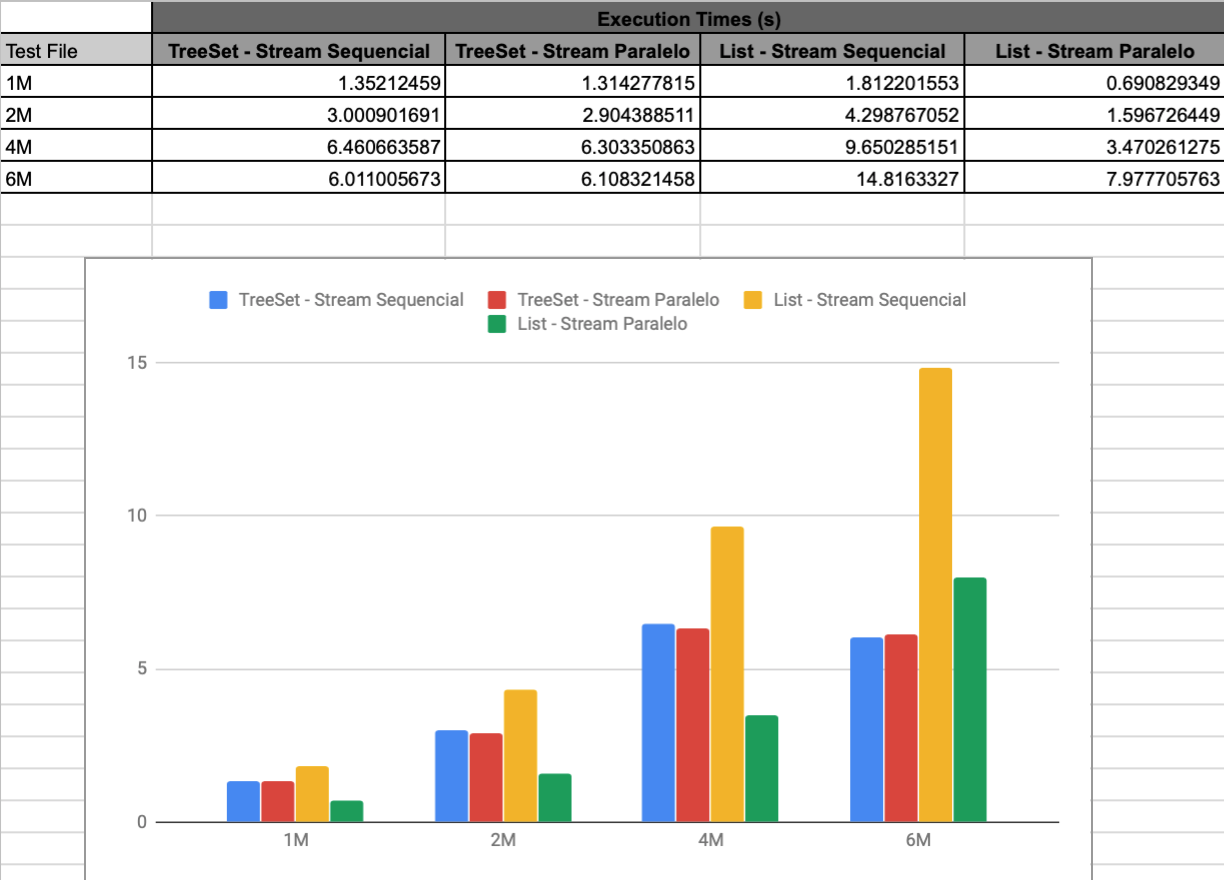
\includegraphics[width=10cm]{Pictures/T2.png}
    \caption{Benchmark T2}
\end{figure}
Como é possível observar, o recurso a \texttt{Lists} aliadas a \texttt{Streams} paralelas
permite obter os melhores resultados até 6 milhões de elementos. Por outro lado, as implementações com \texttt{TreeSets} exibem resultados semelhantes, algo que pode ser justificado pela complexidade desta estrutura de dados que exige sincronização entre \textit{threads} no caso das \texttt{Streams} paralelas, algo que não se verifica nas 
\texttt{Lists} que apresentam bom grau de paralelismo. Este facto leva a uma perda de
\textit{performance} significativa.

\newpage
\subsection{Benchmark T3}
Este \textit{benchmark} consistia em remover valores duplicados do conjunto de transações a tratar. 
A partir da imagem em baixo apresentada podemos concluir que remover valores duplicados recorrendo a \texttt{Lists} é bastante ineficiente comparado com os outros mecanismos analisados.

\begin{figure}[H]
    \centering
    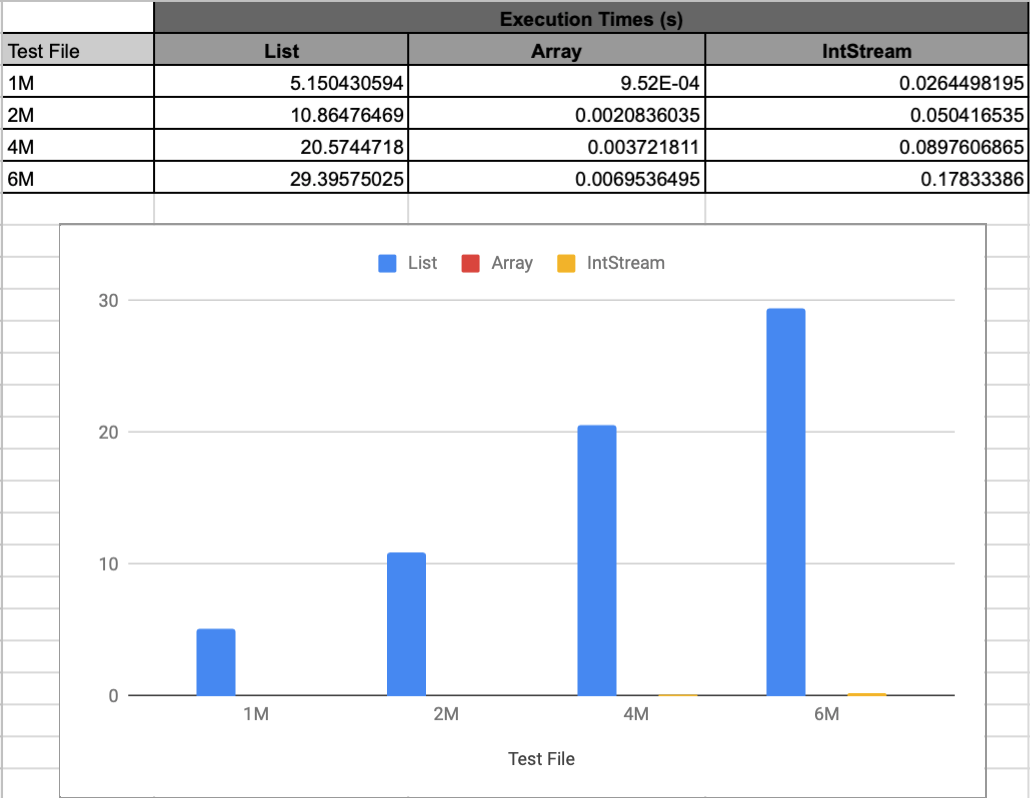
\includegraphics[width=10cm]{Pictures/T3.png}
    \caption{Benchmark T3}
\end{figure}

Sendo assim, passamos a analisar e comparar os resultados obtidos com \texttt{Arrays} e \texttt{IntStream}.

\begin{figure}[H]
    \centering
    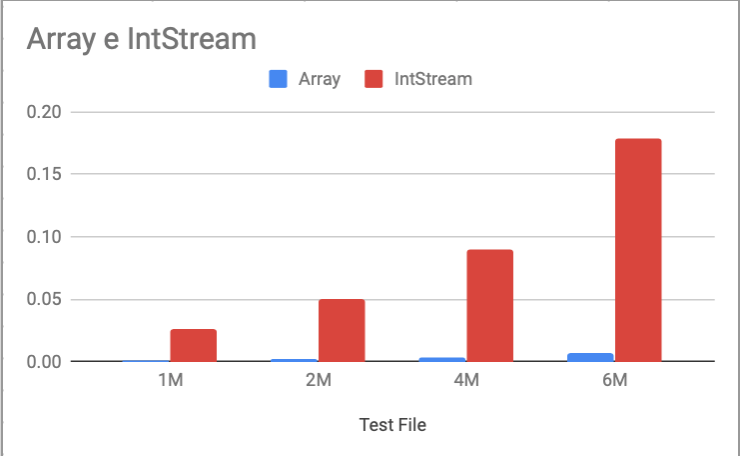
\includegraphics[width=10cm]{Pictures/T3_2.png}
    \caption{Benchmark T3: IntStream vs. Array}
\end{figure}

Apesar de \texttt{IntStream} ser um tipo de stream especializado e obter resultados de tempo bastante inferiores aos obtidos com \texttt{Lists}, apresenta resultados piores que o tempo de remoção de duplicados com o recurso a um \texttt{Array}. Enquanto que o \texttt{Array} utiliza um tipo primitivo, tende a ser mais rápido e melhor a \textit{performance} face a uma estrutura de dados que utiliza a classe \textit{Integer}, que é o caso dos \texttt{Lists} e \texttt{Arrays} utilizados neste \textit{benchmark}. Um objeto do tipo \texttt{Integer} exige \textit{Garbage collection}, ao passo que para o tipo primitivo \texttt{int} o mesmo não é necessário, tendo consequências lógicas na \textit{performance} do programa.

\newpage
\subsection{Benchmark T4}
\label{T4}
A \textit{benchmark} 4 realiza a multiplicação de valores do tipo \texttt{Double} recorrendo para isso a diferentes mecanismos:
\begin{itemize}
    \item \texttt{static method}:
        \begin{lstlisting}
        private static double method_multiplication (double number_1, double number_2){
            return number_1 * number_2;
        } 
        \end{lstlisting}
    \item \texttt{BiFunction}:
        \begin{lstlisting}
        BiFunction<Double, Double, Double> bi_multiplication = (x, y) -> {      
            return x * y;
        }; 
        \end{lstlisting}
    \item expressão lambda:
        \begin{lstlisting}
        Function<Double, Function<Double,Double>> lambda_mul = x -> y -> x * y; 
        \end{lstlisting}
\end{itemize}

\begin{figure}[H]
    \centering
    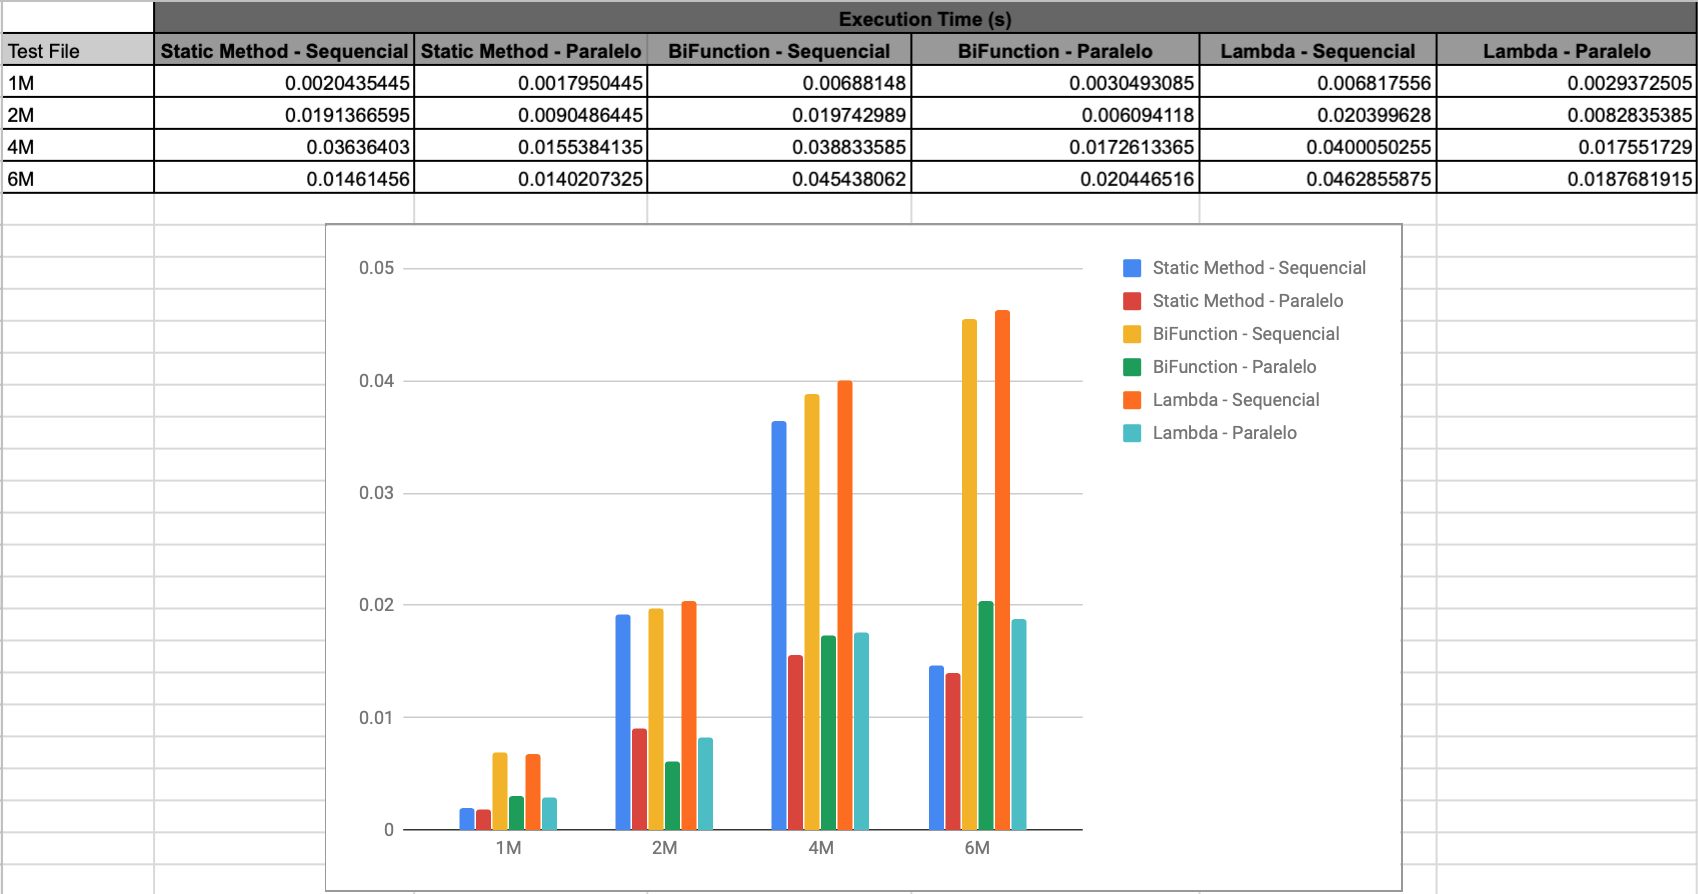
\includegraphics[width=15cm]{Pictures/T4.png}
    \caption{Benchmark T4}
\end{figure}
Como se pode observar, a diferença entre as implementações que recorrem a \textit{interfaces} funcionais (\texttt{BiFunction} e \texttt{lambda(Function)}) e \texttt{static method} é negligenciável, apesar da abstração existente para permitir 
o uso de expressões lambda como se de dados se tratassem. Isto permite concluir que o uso de expressões lambda permite maior legibilidade e agilidade de desenvolvimento sem comprometer
a \textit{performance} das aplicações.
\newpage
\subsection{Benchmark T5}
A \textit{benchmark} 5, de forma semelhante à \textit{benchmark} 2, envolve a utilização de \texttt{TreeSets} e \texttt{Lists} aliadas a \texttt{Streams} paralelas e sequenciais para ordenação de transações.

\begin{figure}[H]
    \centering
    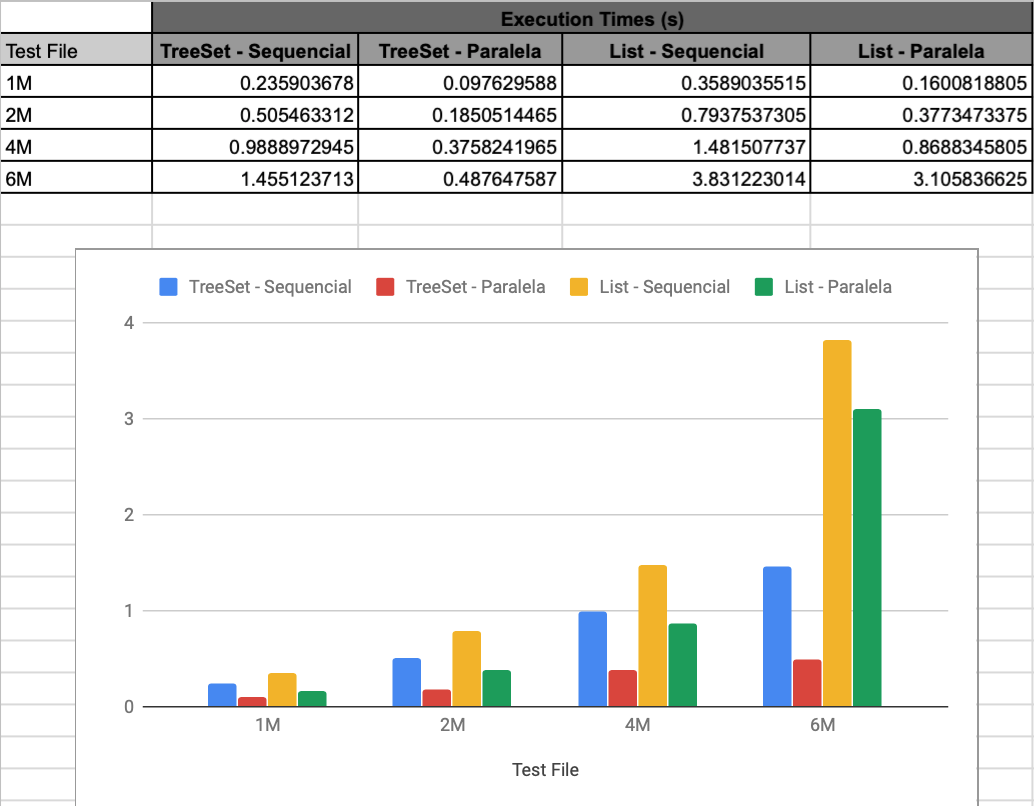
\includegraphics[width=12cm]{Pictures/T5.png}
    \caption{Benchmark T5}
\end{figure}

Face aos valores obtidos através destes testes efetuados, conseguimos depreender que a melhor \textit{performance} é obtida através da utilização de \texttt{TreeSet} com recurso a \texttt{Streams} paralelas.
Ao passo que um \texttt{TreeSet} utiliza as suas caraterísticas expectáveis no que diz respeito à ordenação de dados inseridos, no caso do uso de operações intermédias \textit{stateful} (com estado interno), como o \texttt{sorted()}, a manutenção deste estado implica custos na \textit{performance}, como acontece ao utilizarmos as \texttt{Streams} com \texttt{Lists}. Sendo assim, é expectável que a ordenação com recurso a \texttt{TreeSet} apresente melhores resultados que com recurso a \texttt{Lists}. 

\newpage
\subsection{Benchmark T6}
A \textit{benchmark} 6 pretende comparar a diferenças nas implementações entre
JAVA 7 e Java 8 para a criação de tabelas com transações catalogadas por Mês, Dia e Hora.
Estas diferenças nas versões refletem-se no uso de iteradores como \texttt{Iterator} e 
\texttt{forEach} para JAVA 7 ao invés de \texttt{Streams} paralelas e sequenciais no caso de Java 8.
\begin{figure}[H]
    \centering
    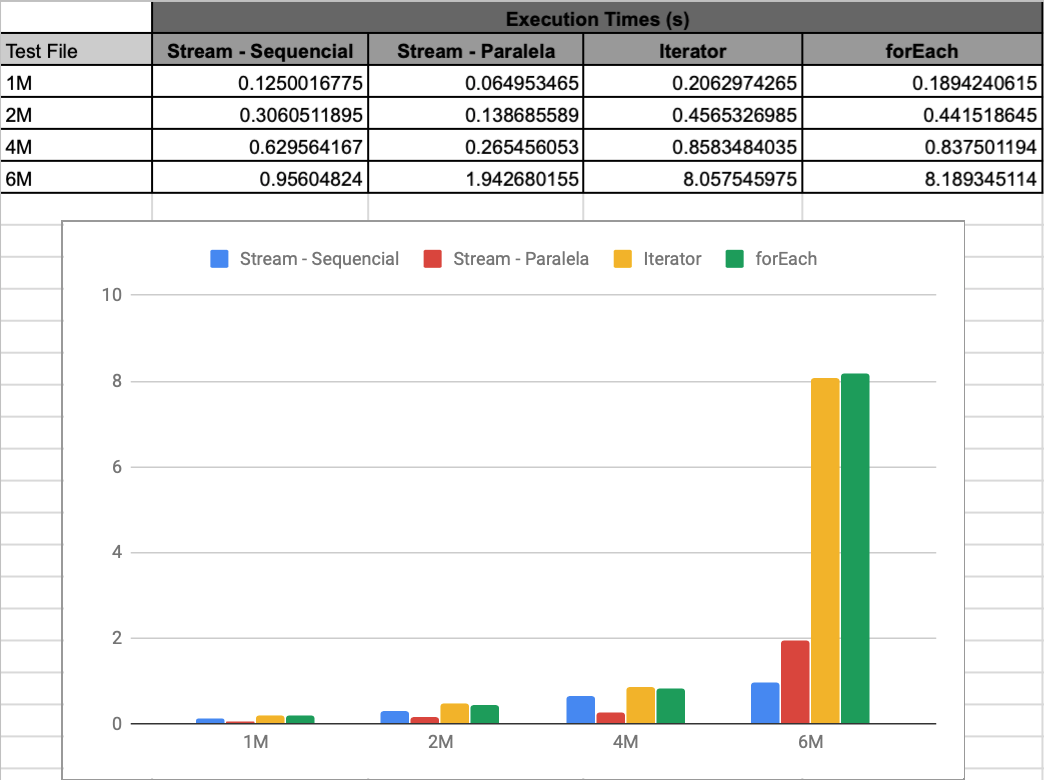
\includegraphics[width=15cm]{Pictures/T6.png}
    \caption{Benchmark T6}
\end{figure}
Percebemos que a utilização de \texttt{Streams} tende a obter melhores resultados que o recurso à interface \texttt{Iterator} ou ao mecanismo \texttt{forEach} (estes dois últimos tendem a apresentar resultados semelhantes ao longo dos testes). Ao passo que o \texttt{Iterator} e o mecanismo \texttt{forEach} são iteradores externos e, sendo assim, cabe ao programador a responsabilidade de otimizar a execução e uso dos mesmos, em sentido contrário, os \texttt{Streams}(iterador interno) fazem parte de uma biblioteca otimizada e que tenta adaptar-se aos dados a tratar e ao \textit{hardware} da máquina em causa, por forma a extrair o máximo desempenho de ambos.

\newpage
\subsection{Benchmark T7}
O objetivo deste \textit{benchmark} passa por calculcar a soma do valor das transações a processar utilizando duas estruturas de dados, \texttt{Lists} e \texttt{Spliterator}, recorrendo ao \texttt{forEach} do Java7 e ao uso de \texttt{Streams} sequenciais e paralelas. 
\begin{figure}[H]
    \centering
    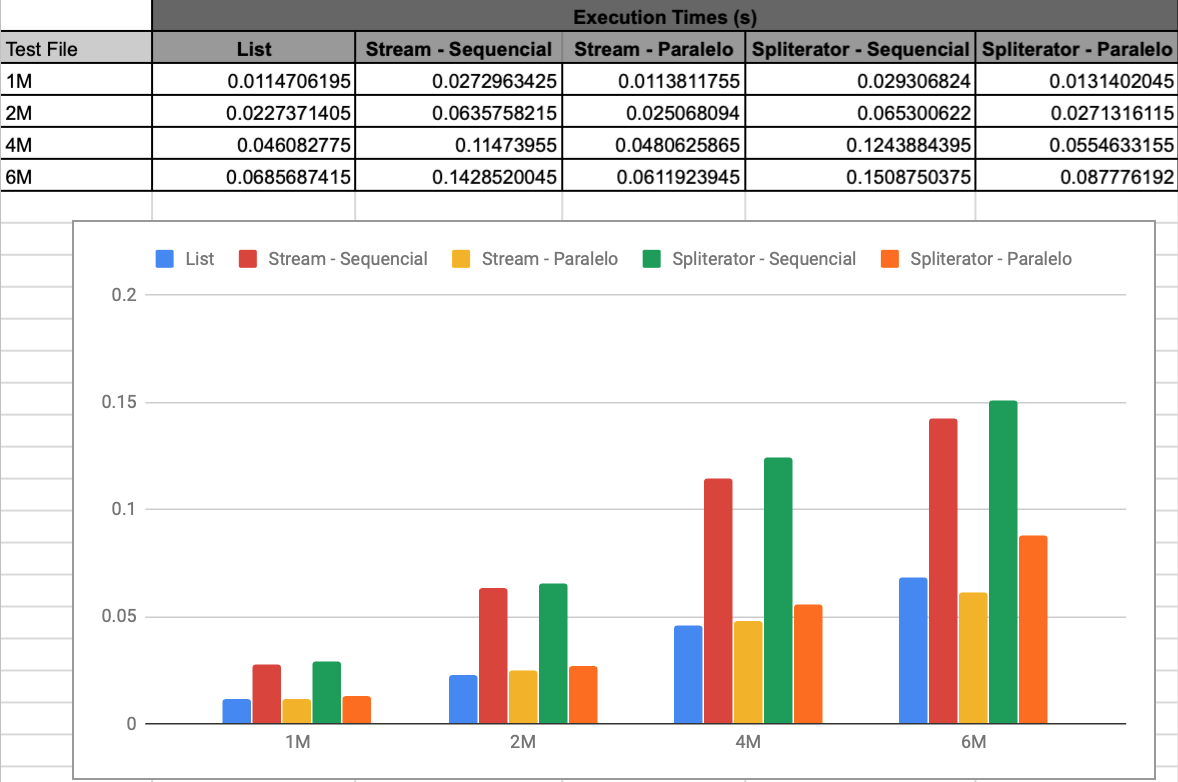
\includegraphics[width=15cm]{Pictures/T7.png}
    \caption{Benchmark T7}
\end{figure}
Verifica-se que os piores resultados ao longo dos testes efetuados são obtidos através da utilização de \texttt{Streams} sequenciais, tanto com o uso de \texttt{Lists} como de \texttt{Spliterators}. A diferença destes resultados para os obtidos com \texttt{Streams} paralelas (tanto em \texttt{Lists} como \texttt{Spliterator}) pode justificar-se pelo facto do tipo de operação (calcular um máximo) ser um processo facilmente paralizável. Para além disto, a utilização do \texttt{forEach} do Java7 apresenta também resultados bastante bons, face à simplicidade da operação em causa neste contexto e devido ao facto da operação
\texttt{max} usada em \texttt{Streams} ser \textit{Stateful}.

\newpage
\subsection{Benchmark T8}
A \textit{benchmark} 8 consiste em determinar a transação com o valor mais elevado efetuada num dado dia entre as 16 e as 22 horas.
São comparadas, para este processo, três implementações distintas, a primera com recurso ao iterador \texttt{forEach} do Java 7, e as restantes com recurso a \texttt{Streams} sequenciais e paralelas.
\begin{figure}[H]
    \centering
    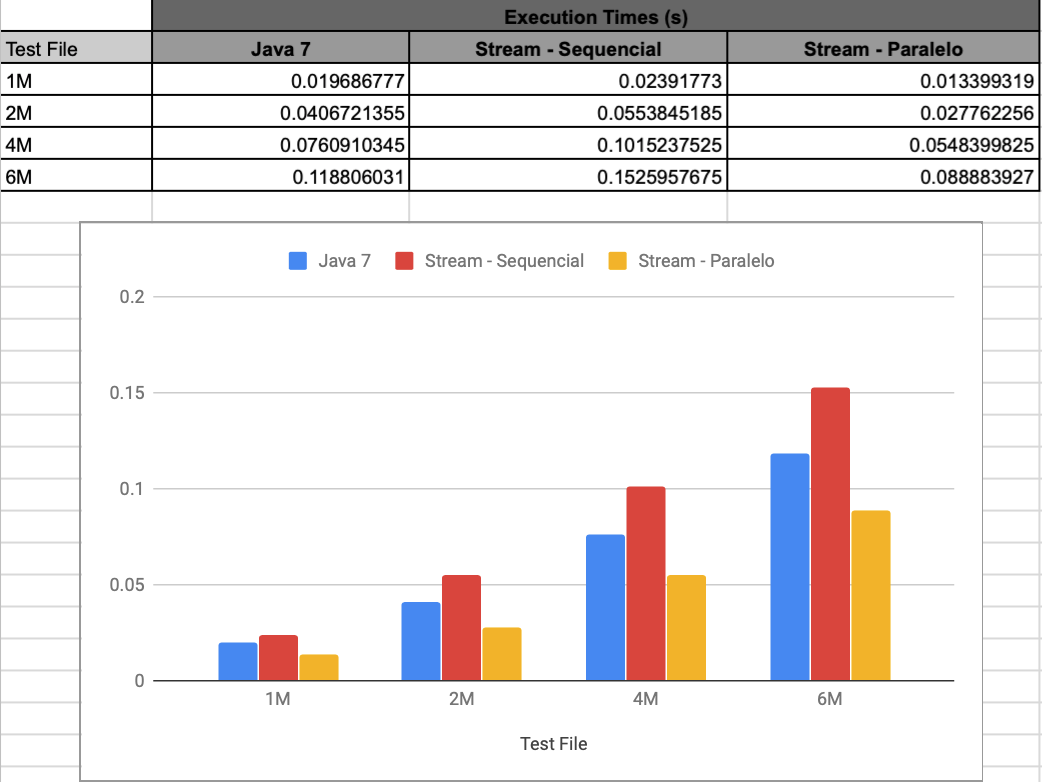
\includegraphics[width=15cm]{Pictures/T8.png}
    \caption{Benchmark T8}
\end{figure}
A operação de filtragem é inerentemente paralela, como tal, e em concordância com os resultados, o recurso a \texttt{Streams} paralelas apresenta melhores tempos de execução.
Por outro lado a falta de \textit{peformance} no caso de \texttt{Streams} sequencias face à versão Java 7 com iterador \texttt{forEach} pode ser justificada pelo custo de 
inicializar a \texttt{Stream} que não existe no caso do \texttt{forEach}.

\newpage
\subsection{Benchmark T9}
O intuito deste \textit{benchmark} era construir uma lista, em que cada elemento da lista corresponde à lista de transações realizadas numa semana. Sendo o objetivo final calcular o total faturado em cada semana , comparando os resultados temporais da codificação em Java 7 (\texttt{forEach}) e em Java 8 com \texttt{Streams} sequenciais e paralelas.
\begin{figure}[H]
    \centering
    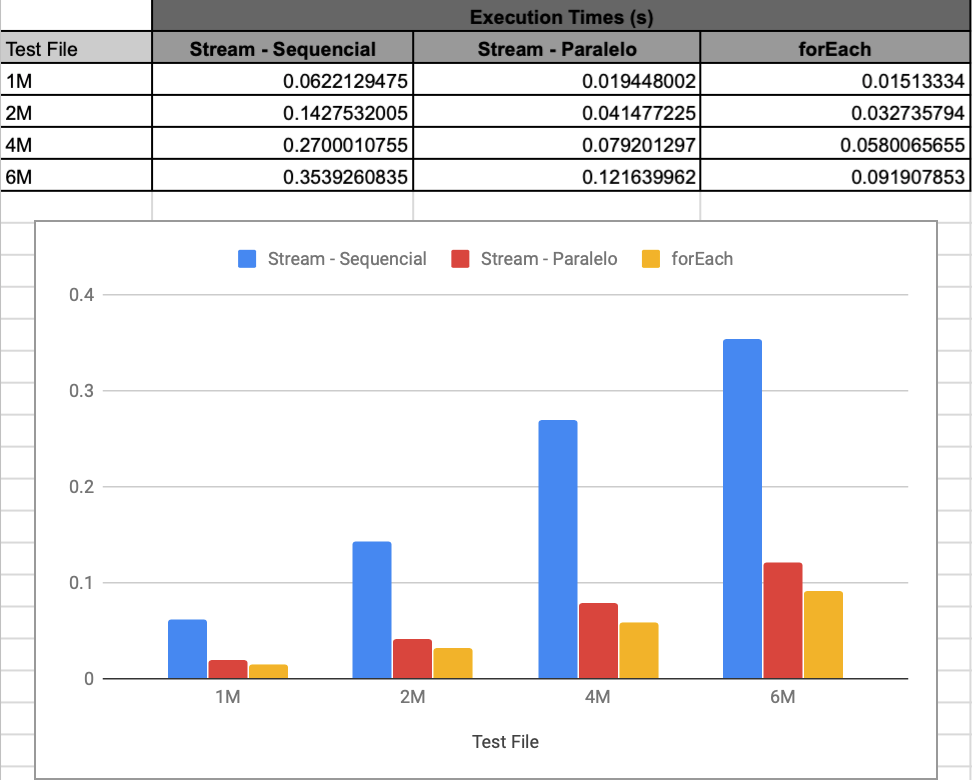
\includegraphics[width=15cm]{Pictures/T9.png}
    \caption{Benchmark T9}
\end{figure}
Pode-se verificar que os resultados em \texttt{Streams} sequenciais são significativamente piores motivado pelo peso envolvido na criação da \texttt{Stream}. Por 
outro lado, no caso da \texttt{Stream} paralela, a diferença para o iterador \texttt{forEach} é consideravelmente inferior, algo motivado pelo facto da operação de 
soma ser facilmente paralelizável. No entanto, o facto de se tratar de uma \texttt{Stream} paralela (com modelo \textit{Fork-and-Join}) exige sincronização entre 
\textit{threads} levando à deterioração da \textit{performance}.

\newpage
\subsection{Benchmark T10}
Na \textit{benchmark} 10 pretende-se construir uma tabela, em que cada mês corresponde ao valor total de IVA a pagar nesse mês. O objetivo é comparar as soluções para Java 7 e Java 8, utilizando \texttt{forEach} na codificação de Java 7 e \texttt{Streams} sequenciais e paralelas na codificação de Java 8.
\begin{figure}[H]
    \centering
    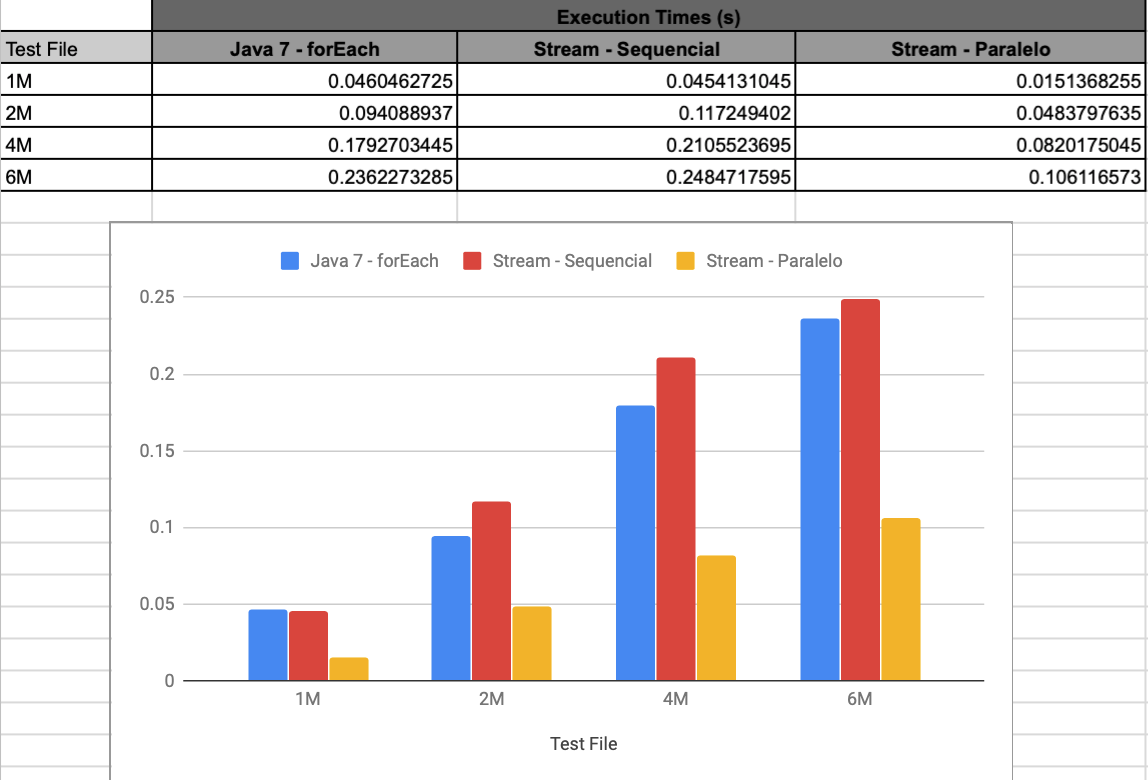
\includegraphics[width=15cm]{Pictures/T10.png}
    \caption{Benchmark T10}
\end{figure}

As soluções com a utilização de \texttt{Stream} sequencial revelam-se as piores mas com diferença pouco significativa em relação à solução com recurso a \texttt{forEach}. Já os resultados da \texttt{Stream} paralela denotam-se muito mais eficientes. Isto vem de acordo com o esperado, visto se tratarem de operações independentes, perfeitas para a utilização de paralelismo.
\newpage
\subsection{Benchmark T11}
A \textit{benchmark} 11 consistia em comparar, para uma das \textit{benchmarks} anteriormente apresentadas(sec. \ref{T4}), a diferença de \textit{performance} observada entre Java 8 e Java 9.
\begin{figure}[H]
    \centering
    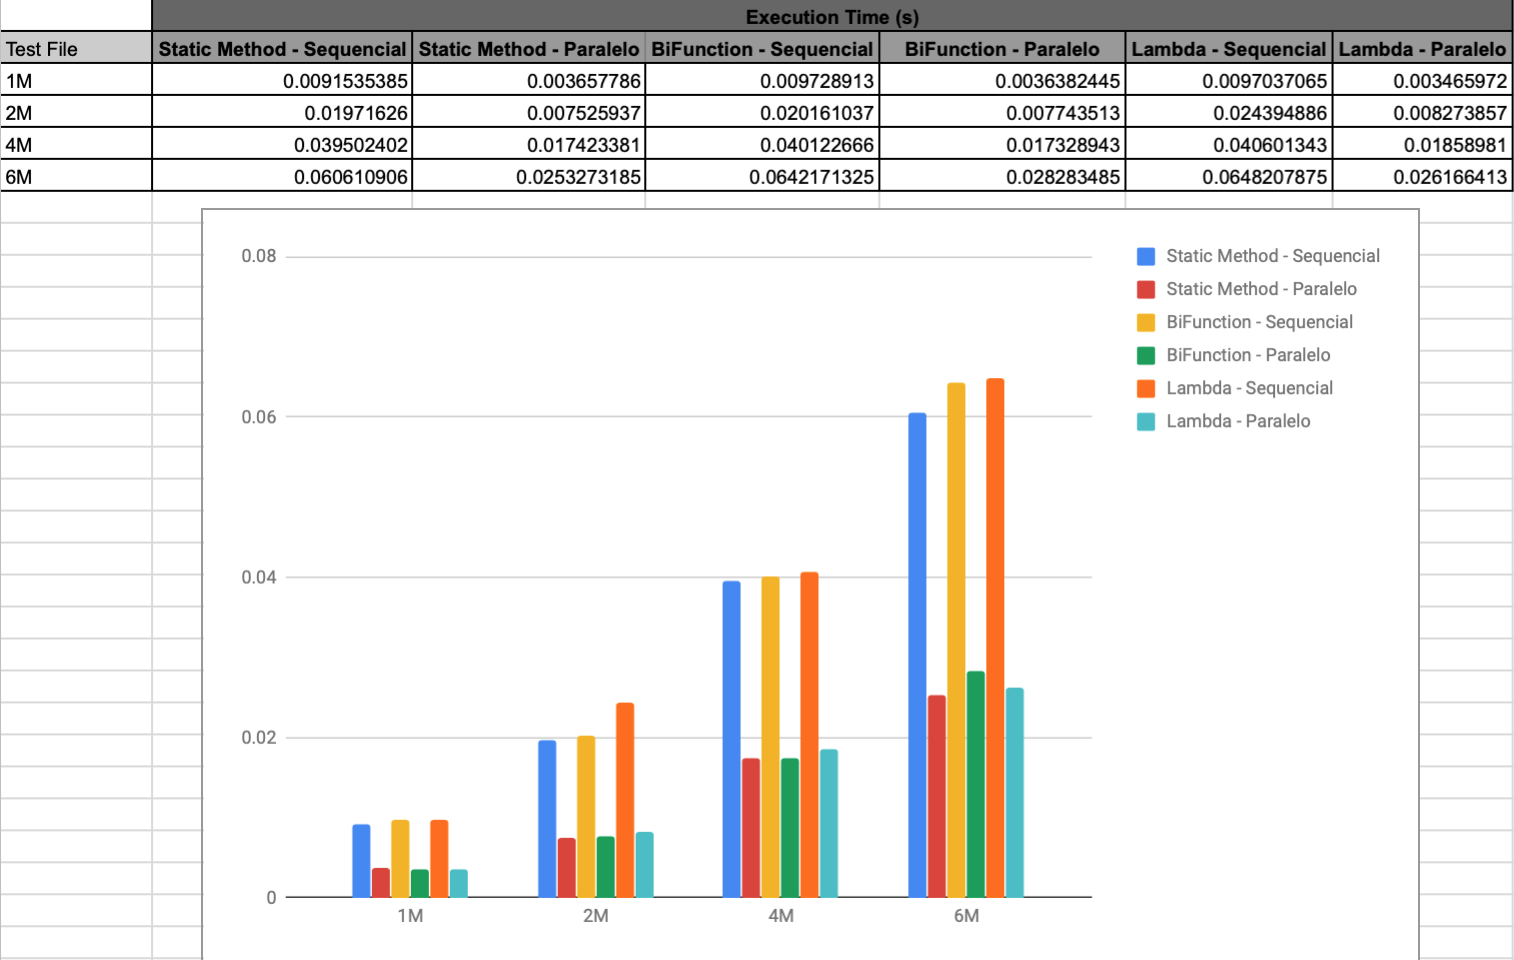
\includegraphics[width=15cm]{Pictures/T11_8.png}
    \caption{Benchmark 11: Java 8}
\end{figure}


\begin{figure}[H]
    \centering
    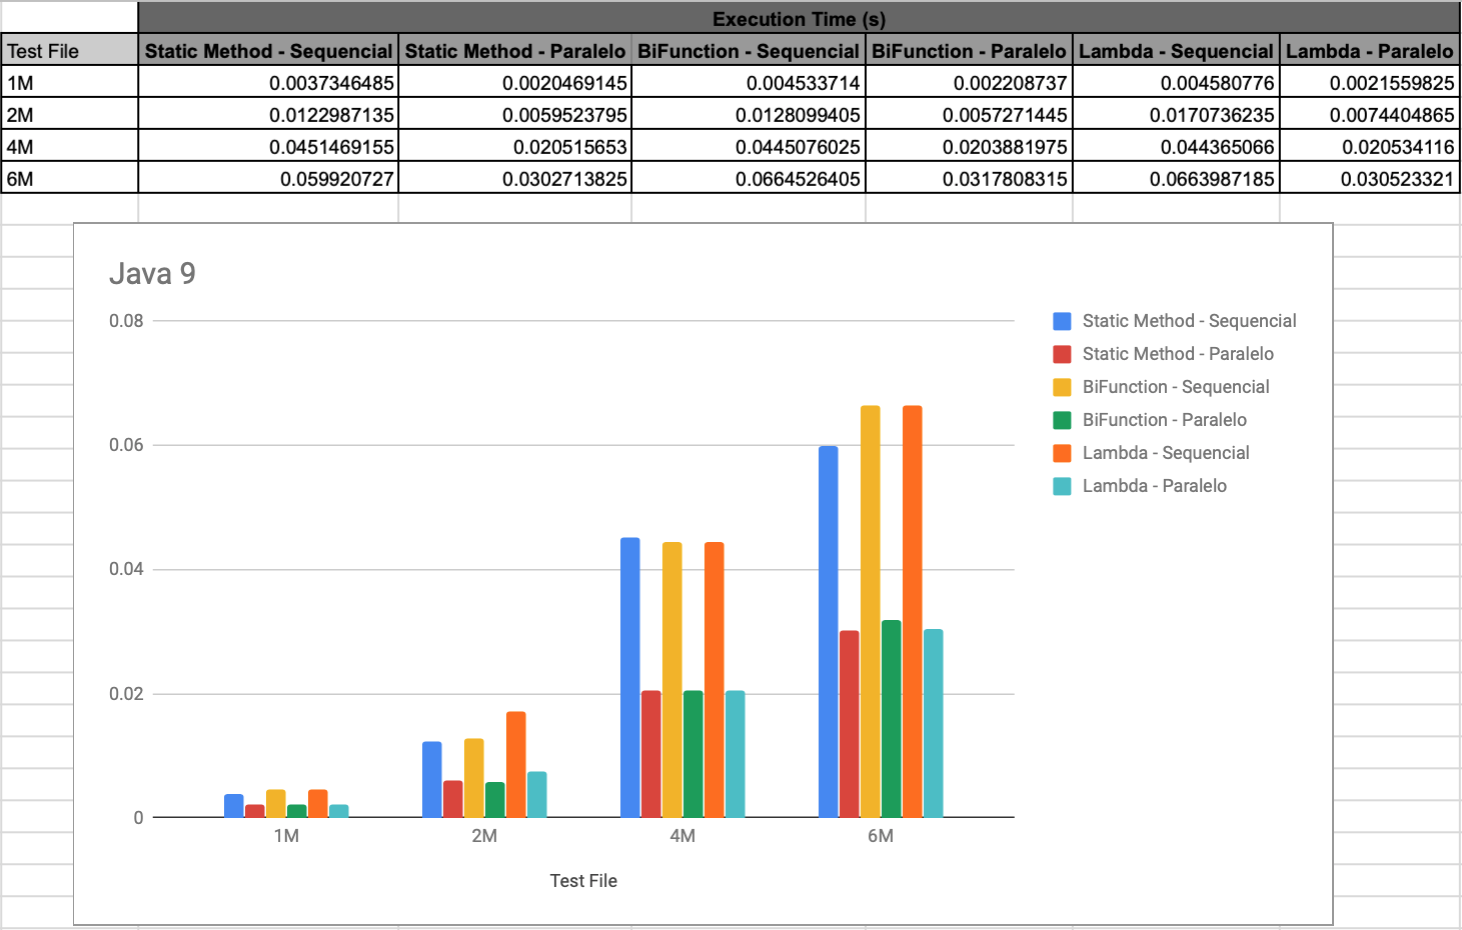
\includegraphics[width=15cm]{Pictures/T11_9.png}
    \caption{Benchmark 11: Java 9}
\end{figure}
Os dados obtidos não permitem observar diferenças significativas entre as duas versões de Java: 8 e 9. 
É interessante realçar que, no caso das implementações paralelas, existe um pequeno aumento na \textit{performance} para os data sets de tamanho menor, algo que pode
ser explicado por uma melhor gestão do paralelismo por parte da JVM em versões mais recentes que permite colmatar o impacto desta (gestão) no desempenho das aplicações.



\newpage
\subsection{Benchmark T12}

Neste \textit{benchmark} pretende-se testar a diferença de \textit{performance} entre tabelas feitas com recurso a \texttt{Map} e \texttt{ConcurrentMap}, em Java 8 e 9. Para isso é pedido para criar uma tabela que associa a cada nº de caixa uma tabela contendo para cada mês as transações dessa caixa. Posteriormente pretende-se calcular o total faturado por caixa. 
\begin{figure}[H]
    \centering
    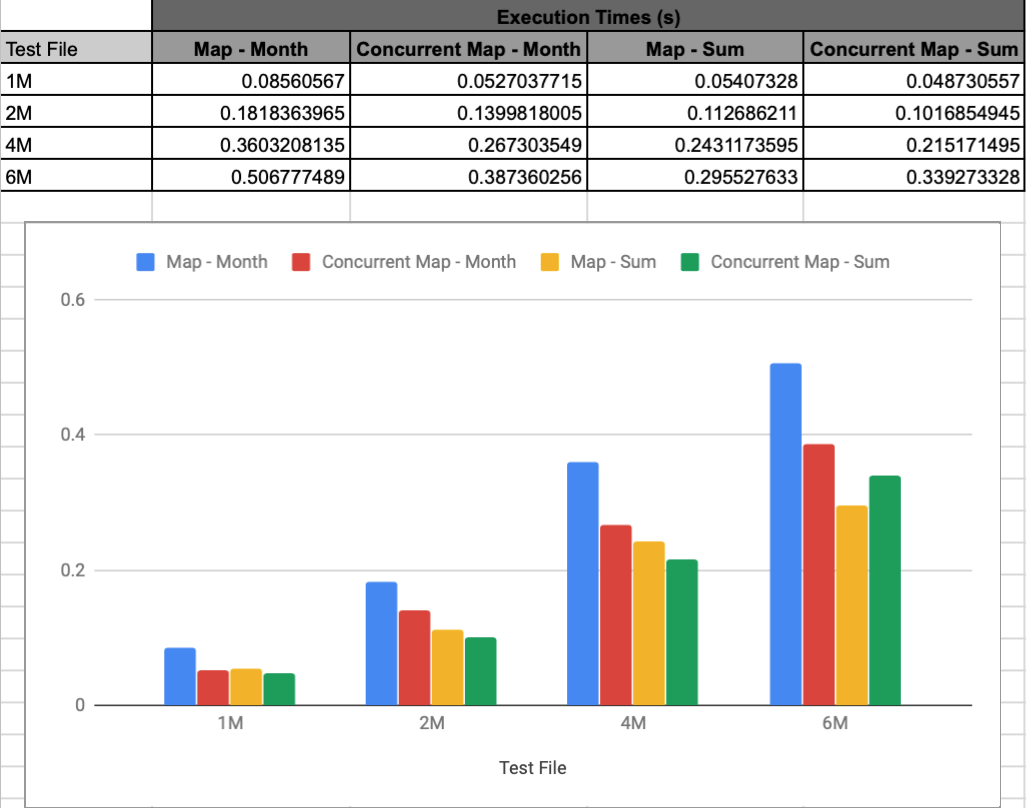
\includegraphics[width=15cm]{Pictures/T12_8.png}
    \caption{Benchmark 12: Java 8}
\end{figure}
Pode-se notar que a \textit{performance} da construção e operação de soma com as tabelas usando o \texttt{ConcurrentMap} apresenta melhores resultados.
\begin{figure}[H]
    \centering
    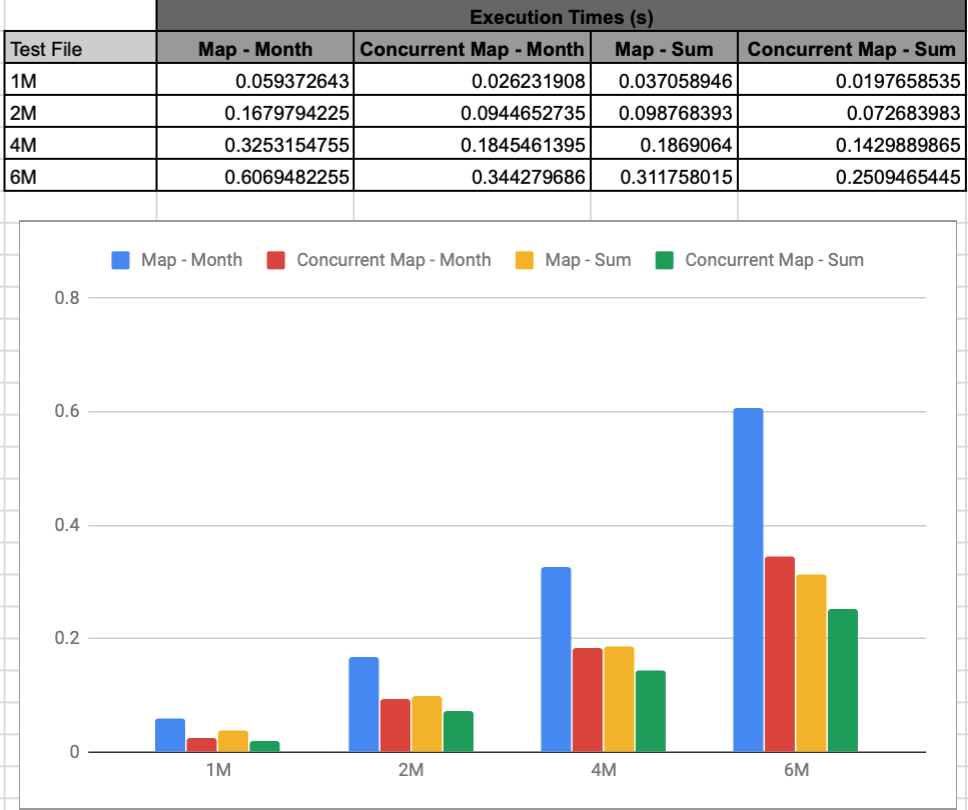
\includegraphics[width=15cm]{Pictures/T12_9.png}
    \caption{Benchmark 12: Java 9}
\end{figure}
Em Java 9, os resultados com \texttt{ConcurrentMap} apresentam sempre melhores tempos.
Pode-se concluir que para este \textit{benchmark} o uso de \texttt{ConcurrentMap} mostrou-se ser mais eficiente, pois as operações são feitas paralelamente, o que é apenas benéfico ao nivel de \textit{performance} derivado de se tratar de operações independentes.

\section{Conclusão}
Observando os dados analisados/recolhidos é possível concluir que o uso de \texttt{Streams} de Java nem sempre se apresenta como a melhor alternativa, apesar da sua facilidade de uso. Por outro lado, e em contraste, é também evidente que deve ser sempre priorizado o uso de tipos primitivos (\texttt{int, double, long,...}) face 
aos seus homólogos no caso dos objetos, isto porque os primeiros não apresentam uma utilização de memória tão elevada como os segundos, levando a uma pressão menor 
sobre o \textit{Garbage Collector} da JVM(\textit{Java Virtual Machine}). É ainda importante referir que, dado o modelo \texttt{Fork-and-Join} das \texttt{Streams} 
paralelas de Java, o seu uso deve ser ponderado dado que a gestão/sincronização das \textit{threads} envolvidas pode ter um impacto negativo na \textit{performance} que negue o benefício do uso \cite{parallel_considerations}.
Uma falha que pode ser apontada ao presente trabalho seria a ausência de realização de testes com 8 milhões de transações, ausência esta que é justificada pela 
incapacidade de correr os testes com este \textit{data set} na máquina escolhida, mesmo alterando parâmetros como o tamanho da \textit{heap} da JVM
(\textbf{i.e.}\texttt{-Xmx 4gb}). No entanto, dada a dimensão das amostras recolhidas, consideramos que os resultados obtidos resultariam em conclusões semelhantes às
apresentadas.

\printbibliography

\end{document}
